% 2007 年安徽卷理科第 9 题：双曲线 x^2/a^2-y^2/b^2=1、以 O 为圆心 |OF_1| 为半径的圆，
%   圆与双曲线左支交于 A、B，且 F_2AB 为等边三角形。
% 来源 PDF：gaokaomath-src/普通高考/2007/2007安徽理.pdf
% SHA-256：3f85f741d3b3790a308d698e4826ab196259643a8d40de12753c61cc6a9d2f0b
% 原页：2007安徽理.pdf 第 1 页（A3 三栏）第 2 栏，书页码 347，图在第 9 题题干下方。
% 重绘依据：按题设 e=1+sqrt3 的真实配置取 c=1、a=1/2（b=sqrt3/2），此时圆与左支交点
%   恰为 A(-1/2,sqrt3/2)、B(-1/2,-sqrt3/2)，AB=sqrt3=F_2A=F_2B，等边三角形严格成立。
%   画 x 轴（带箭头）、过 O 的 y 轴（原图无箭头无标注）、圆、左右两支、线段 F_2A、F_2B、AB。
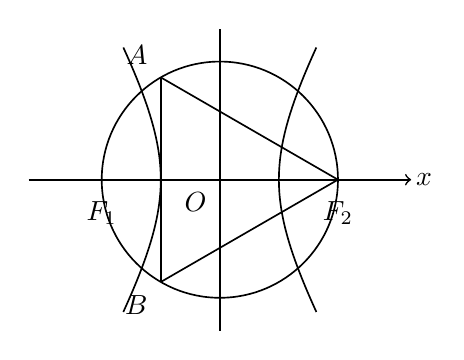
\begin{tikzpicture}[scale=1.5, semithick,
  every node/.style={inner sep=1.5pt}]
  % 坐标轴
  \draw[->] (-1.62,0) -- (1.62,0) node[anchor=west] {$x$};
  \draw (0,-1.28) -- (0,1.28);
  % 圆
  \draw (0,0) circle (1);
  % 双曲线左右两支：x = ±(1/2)sqrt(1+y^2/(3/4))
  \draw plot[domain=-1.12:1.12, samples=90]
    ({-0.5*sqrt(1+\x*\x/0.75)}, \x);
  \draw plot[domain=-1.12:1.12, samples=90]
    ({0.5*sqrt(1+\x*\x/0.75)}, \x);
  % 交点与焦点
  \coordinate (O)  at (0,0);
  \coordinate (A)  at (-0.5,0.8660254);
  \coordinate (B)  at (-0.5,-0.8660254);
  \coordinate (F1) at (-1,0);
  \coordinate (F2) at (1,0);
  \draw (A) -- (F2) -- (B);
  \draw (A) -- (B);
  \node[anchor=south east] at ([xshift=-2pt,yshift=2pt]A) {$A$};
  \node[anchor=north east] at ([xshift=-2pt,yshift=-2pt]B) {$B$};
  \node[anchor=north] at ([yshift=-4pt]F1) {$F_1$};
  \node[anchor=north] at ([yshift=-4pt]F2) {$F_2$};
  \node[anchor=north east] at ([xshift=-2pt,yshift=-2pt]O) {$O$};
\end{tikzpicture}
